%%%%%%%%%%%%%%%%%%%%%%%%%%%%%%%%%%%%%%%%%
% a0poster Landscape Poster
% LaTeX Template
% Version 1.0 (22/06/13)
%
% The a0poster class was created by:
% Gerlinde Kettl and Matthias Weiser (tex@kettl.de)
% 
% This template has been downloaded from:
% http://www.LaTeXTemplates.com
%
% License:
% CC BY-NC-SA 3.0 (http://creativecommons.org/licenses/by-nc-sa/3.0/)
%
%%%%%%%%%%%%%%%%%%%%%%%%%%%%%%%%%%%%%%%%%

%----------------------------------------------------------------------------------------
%	PACKAGES AND OTHER DOCUMENT CONFIGURATIONS
%----------------------------------------------------------------------------------------

\documentclass[a0,landscape]{a0poster}

\usepackage{multicol} % This is so we can have multiple columns of text side-by-side
\columnsep=100pt % This is the amount of white space between the columns in the poster
\columnseprule=3pt % This is the thickness of the black line between the columns in the poster

\usepackage[svgnames]{xcolor} % Specify colors by their 'svgnames', for a full list of all colors available see here: http://www.latextemplates.com/svgnames-colors

\usepackage{times} % Use the times font

\usepackage{graphicx} % Required for including images
\graphicspath{{figures/}} % Location of the graphics files
\usepackage{booktabs} % Top and bottom rules for table
\usepackage[font=small,labelfont=bf]{caption} % Caption provides ways to customise the captions in floating environments like figure and table, e.g., rotating captions, side­ways cap­tions, etc.
\usepackage{amsfonts, amsmath, amsthm, amssymb} % For math fonts, symbols and environments
\usepackage{wrapfig} % Allows wrapping text around tables and figures

\begin{document}

%----------------------------------------------------------------------------------------
%	POSTER HEADER 
%----------------------------------------------------------------------------------------

% The header is divided into three boxes:
% The first is 55% wide and houses the title, subtitle, names and university/organization
% The second is 25% wide and houses contact information
% The third is 19% wide and houses a logo for your university/organization or a photo of you
% The widths of these boxes can be easily edited to accommodate your content as you see fit

% \linewidth refers to the width of text in the current environment

\begin{minipage}[b]{0.55\linewidth}
  \veryHuge \color{NavyBlue} \textbf{Outta Control: Laws of Semantic Change and Inherent Biases in Word Representation Models} \color{Black}\\ % Title
  \Huge \textit{Dubossarsky et al. (2017)}\\[1cm] % Subtitle
  \huge \textbf{John Smith \& James Smith}\\ % Author(s)
  \huge IMS, Universität Stuttgart \\ % University/organization
\end{minipage}
%
\begin{minipage}[b]{0.25\linewidth}
  \color{DarkSlateGray}\Large \textbf{Contact Information:}\\
  Institut für Maschinelle Sprachverarbeitung\\ % Address
  Universität Stuttgart\\
  Germany\\\\
  Email: \texttt{john@LaTeXTemplates.com}\\ % Email address
\end{minipage}
%
\begin{minipage}[b]{0.19\linewidth}
  
\includegraphics[width=20cm]{logo.png} % Logo or a photo of you, adjust its dimensions here
\end{minipage}

\vspace{1cm} % A bit of extra whitespace between the header and poster content

%----------------------------------------------------------------------------------------

\begin{multicols}{4} % This is how many columns your poster will be broken into, a poster with many figures may benefit from less columns whereas a text-heavy poster benefits from more

%----------------------------------------------------------------------------------------
%	ABSTRACT
%----------------------------------------------------------------------------------------

\color{Navy} % Navy color for the abstract

\begin{abstract}

This paper evaluates the validity of previously stated laws of semantic change in literature by applying them on a randomized controlled data set. The claim is that if semantic change can indeed be represented by the theoretical laws as reported in previous literature, their effect should not be seen on a randomized data set, or at least get significantly diminished.

The goal is to specifically analyze these three laws:

\begin{itemize}
  \item The Law of Conformity: Frequency is negatively correlated with semantic change.
  \item The Law of Innovation: Polysemy is positively correlated with semantic change.
  \item The Law of Prototypicality: Prototypicality is negatively correlated with semantic change.
\end{itemize}

\end{abstract}

%----------------------------------------------------------------------------------------
%	INTRODUCTION
%----------------------------------------------------------------------------------------

\color{SaddleBrown} % SaddleBrown color for the introduction

\section*{Introduction}
To understand the ever-changing nature of language, a very popular way to quantify the semantic change for a particular word is to create word vector representations of the word for two different points in time and then measure the cosine distance. This method depends on the choice of model used to calculate the word representations. Since most models use co-occurrence statistics and word frequency, there is an inherent bias present in these models which challenges the ubiquity of the effect of the proposed laws of semantic change.

% The test proposed is fairly simple: The laws should hold for real data but not for random data. Also, if no change in meaning occurs, the laws should not be observed.

%----------------------------------------------------------------------------------------
%	OBJECTIVES
%----------------------------------------------------------------------------------------

\color{DarkSlateGray} % DarkSlateGray color for the rest of the content

%  motivation, related work, materials and methods, experiments, conclusions

% \section*{Motivation}

%----------------------------------------------------------------------------------------
%	MATERIALS AND METHODS
%----------------------------------------------------------------------------------------

\section*{MATERIALS AND METHODS}

%------------------------------------------------

\subsection*{Real Data}
The historical data-set used is Google Books 5-grams of English fiction. Equally sized samples of 10 million 5-grams per year were taken for the period 1900-1999. To account for outliers, uncommon words were removed and the 100,000 most frequent words were used as the vocabulary. Since this data spans an entire century, it is big enough to assume the presence of semantic change, thereby making it appropriate for carrying out the testing process.

\subsection*{Controlled data}
\subsubsection*{Continuously shuffled corpus (Shuffle)}
This corpus tries to distribute the semantic meaning change uniformly across the whole time period of the data. To do this, the 5-grams in the original data were randomly shuffled to achieve a uniform distribution. Any semantic change trends which were previously present should get significantly diminished in this new shuffled corpus and must be attributed to chance.

\subsubsection*{ One synchronous corpus (sample)}
Since the smallest time unit of the dataset is one year, the underlying assumption in all models of semantic change is that no meaning change happens within a single year. Therefore the 10 million 5-grams were randomly subsampled from all the 5-grams of the year 1999 and this process was repeated 30 times. Since this entire corpus comes from a single year, any changes observed in this corpus will be attributed to “noise”.

Figure ~\ref{fig:data} shows an overview of the word distribution in  genuine and shuffled corpus.

\begin{center}\vspace{1cm}
  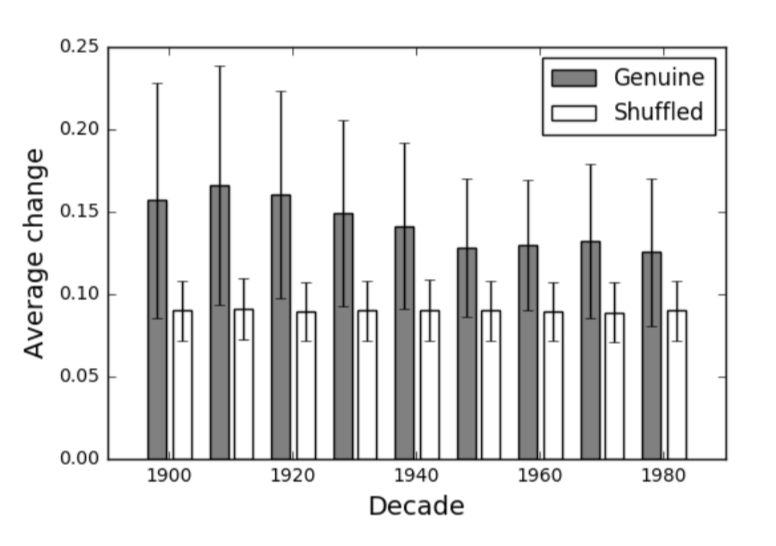
\includegraphics[width=0.8\linewidth]{image3.png}
  \captionof{figure}{\color{Green} Average and Standard Deviation of Change Scores for each Decade}
  \label{fig:data}
\end{center}\vspace{1cm}

\subsection*{Word meaning representations} 
The words in the corpus were mathematically represented in the following ways:
\begin{itemize}
  \item Counts: Co-occurrence counts were collected for all the words in the vocabulary per decade.
  \item PPMI: Sparse square matrices of size equal to that of vocabulary size were created to store the pointwise mutual information (PPMI) scores for each decade. These scores were based on co-occurrence counts of the words.
  \item SVD: The PPMI matrix was reduced into lower dimensions by singular vector decomposition. The resulting embeddings were then aligned with the orthogonal Procrustes method.
\end{itemize}

\begin{center}\vspace{1cm}
  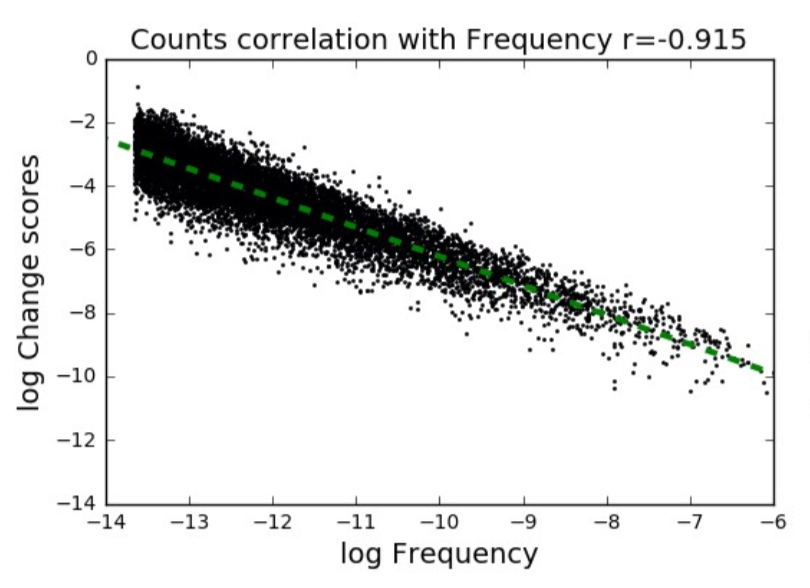
\includegraphics[width=0.8\linewidth]{image2.png}
  \captionof{figure}{\color{Green} Correlation between frequency of words and their change scores for the year 1999}
  \label{fig:wordfreq}
\end{center}\vspace{1cm}
 

%----------------------------------------------------------------------------------------
%	RESULTS 
%----------------------------------------------------------------------------------------

\section*{Results}
\subsection*{Testing the law of Conformity} 

\subsubsection*{Subsample Condition} 
The authors calculated the correlation between frequency of words and their corresponding change scores for the year 1999. Since the assumption was that there is no semantic change within a year, the correlation should be negligible. However, for the word count representation, the correlation was -0.915 while it was -0.295 and -0.793 for PPMI and SVD respectively. This is clearly in violation of the law. The authors also point out that the correlation for SVD is misleading because of the mathematical distortions carried out while reducing the dimensions. Therefore, in principle, the actual correlation must have been lesser than what was observed. However, in any case, the law of conformity is not holding up for the subsample condition. Figure ~\ref{fig:wordfreq} shows the correlation for word frequencies and semantic change in a single year.


\begin{center}\vspace{1cm}
  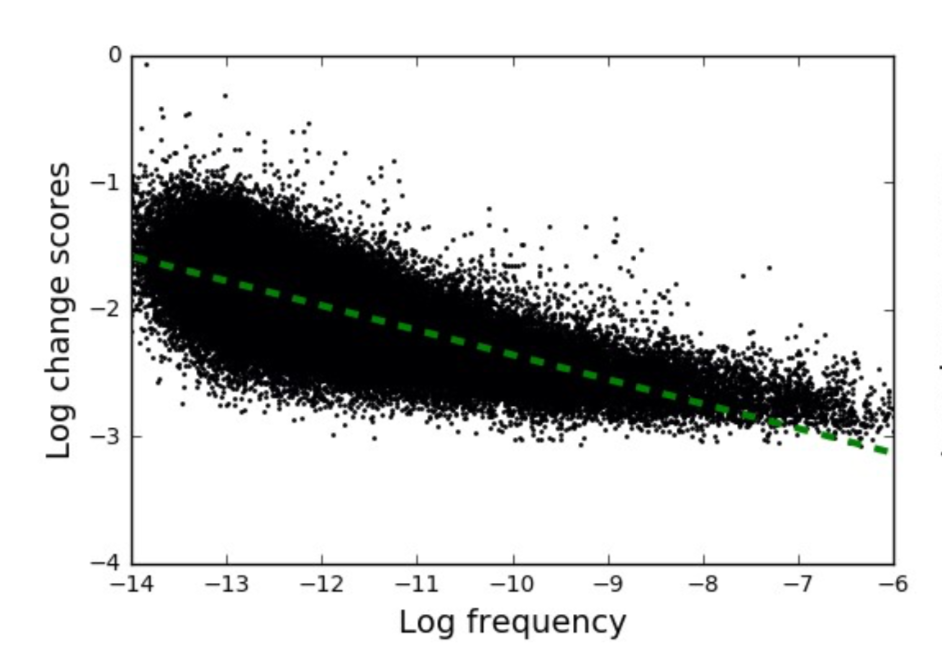
\includegraphics[width=0.8\linewidth]{image7.png}
  \captionof{figure}{\color{Green} Genuine Data}
  \label{fig:genuinedata}
\end{center}\vspace{1cm}

\begin{center}\vspace{1cm}
  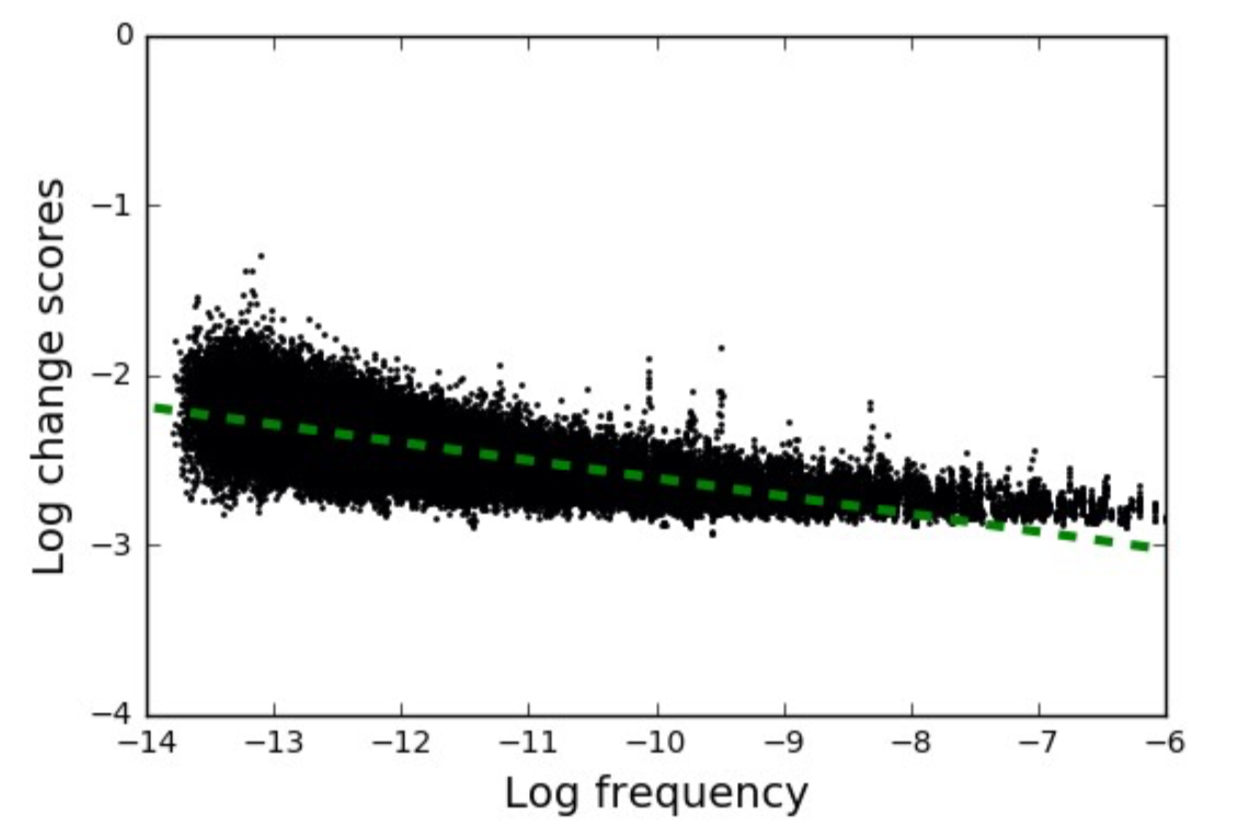
\includegraphics[width=0.8\linewidth]{image5.png}
  \captionof{figure}{\color{Green} Shuffled Data}
  \label{fig:shuffledata}
\end{center}\vspace{1cm}

\subsubsection*{Shuffle Condition} 
Now the correlation was calculated between semantic change scores and frequency for the whole century using the shuffle corpus. In stark contrast to expectations, almost identical correlation coefficients were observed for both the original and the shuffled corpus. This tells us that the effect of frequency is not really as great as has been reported in literature. Figure ~\ref{fig:genuinedata} and ~\ref{fig:shuffledata} illustrate this.


\subsection*{Testing the law of Innovation and Prototypicality}
To test these two laws, the authors did a regression analysis with frequency and polysemy as the independent variables for the law of innovation and frequency and prototypicality for the law of prototypicality. For these models with two predictor variables, the authors compared the the $\beta$ and the explained variance for both the original and shuffled corpus.

Again, contrary to expectations, not much difference was seen between the two corpus. In case of polysemy, the explained variance for PPMI+SVD representations was 68\% and 60\% for original and shuffle respectively. For PPMI representations, these numbers were 9\% and 4\% respectively. This difference is way too less and it can be concluded that the law of innovation is not very strong. The reason according to the paper is that polysemy is highly collinear with frequency and therefore does not make any strong contributions to the two variable regression model.

Similarly for prototypicality for PPMI+SVD representations, the explained variance was 65\% and 60\% for the genuine and shuffle corpus respectively. For PPMI representations, these numbers were 2\% and 0\% respectively.

% Once again, the difference was too low and the law of prototypicality does not seem to be holding up.

% An important point to note is that the models using only PPMI representations explain very insignificant amounts of variance while this is not the case with PPMI+SVD representations. This fact implies that the model of semantic meaning change is highly dependent on the underlying word representation it uses and is not very generalizable, thereby highlighting another major drawback.

%----------------------------------------------------------------------------------------
%	CONCLUSIONS
%----------------------------------------------------------------------------------------

\color{SaddleBrown} % SaddleBrown color for the conclusions to make them stand out

\section*{Conclusions}
The paper showed the failure of three laws of semantic change which had been reported in literature. The extent of the relationship as claimed was not observed when tested with randomized control data. This shows the fragility of the current state of research and points out the vulnerabilities of the mathematics and data used to prove these laws.

The paper also showed that the output of a model of semantic change is often dependent on the word representations it is using. As was seen in subsample case of the law of conformity, different representations provided different correlation values. The authors argue that the representations using count vectors inherently introduce a dependence of word frequency, which then leads to misleading observations.

% The positive aspect is that the paper presented a framework for testing and evaluating the results of a model before it gets generalized.

% This is a very important contribution as testing is something which often gets neglected by people.

\color{DarkSlateGray} % Set the color back to DarkSlateGray for the rest of the content

%----------------------------------------------------------------------------------------
%	REFERENCES
%----------------------------------------------------------------------------------------

\nocite{*} % Print all references regardless of whether they were cited in the poster or not
\bibliographystyle{plain} % Plain referencing style
\bibliography{sample} % Use the example bibliography file sample.bib

%----------------------------------------------------------------------------------------

\end{multicols}

\end{document}
